\section{Experimental Analysis}
\label{sec:experimentdesign}

We performed a set of simulations to evaluate the performance of the heuristic algorithms. The results are illustrated in the next subsections with different metrics.

\subsection{Max Network Throughput} 
The capacity of a network binds with multiple factors, such as gateway placement, routing and also channel assignment. 
Stefano bring the good put in the network without considering the interference as maximum throughput to evaluate the channel assignment ~\cite{avallone2008channel}. However, without considering the interference, the traffic flow in the network is not scheduled.
And to find the best routing associate with channel assignment is out of our scope. 
We would like to calculate the max network capacity as follow.

In a mesh network, the bottleneck of the network are the links around the gateway nodes ~\cite{robinson2010deploying}. 
And any packet transmitted to the wired gateway node is the same. So the best way to get a scheduler maximum throughput is to serve the nodes close to the gateway nodes.
Thus to employ more capacity of the gateway neighbor links, we would like to serve the nodes close to the gateway nodes.
We first serve the node has 1 hop path to the gateway nodes, then choose the path has the least interference on the network and serve the demand as more as possible. Then we satisfy the demand of 2 hop layer nodes and so on, till there is no demand could be satisfied.
This calculation process is kind of routing protocol which help us to reach a scrollable maximum throughput of the network.

We randomly assign demand of mesh nodes with an upper bound, calculate the scalable maximum throughput, and repeat the process 20 times, then output the average maximum throughput for this demand upper bound.
The performance of the two heuristic algorithms and ~\emph{CCA} ~\cite{draves2004routing}, ~\emph{BFSCA}  ~\cite{ramachandran2006interference} in a 30-node regular grid topology with 6MB link capacity
 are shown in figure ~\ref{fig:maxtpt}.

\begin{figure}
%\vspace{-0.0in}
\centering
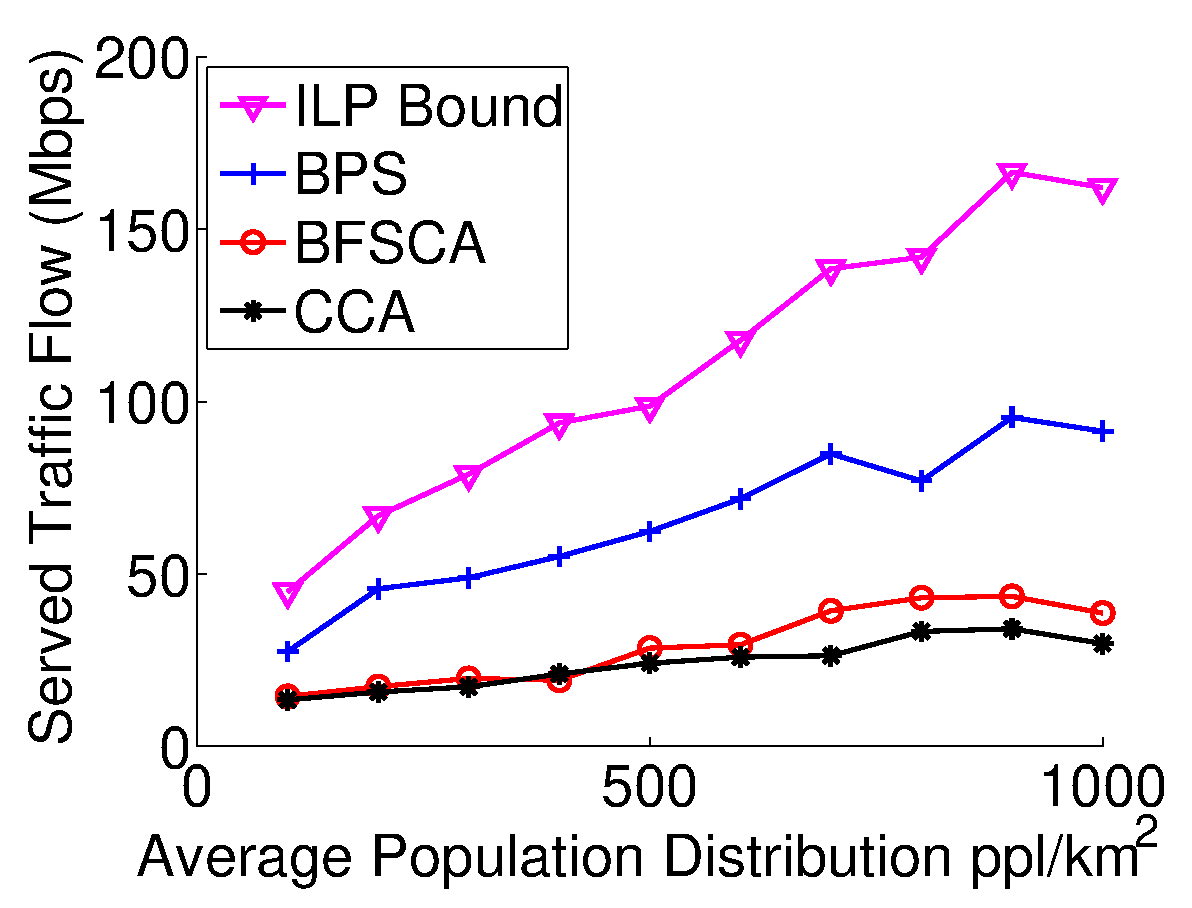
\includegraphics[width=74mm]{figures/maxtpt}
\vspace{-0.1in}
\caption{Max Tpt under Demand Bound}                                                                               
\label{fig:maxtpt}
%\vspace{-0.0in}
\end{figure}

To evaluate the performance in different size of network, we assign the demand of each node $5MB/s$ as demand upper bound, and vary the number of nodes in the regular grid network. The performance of the algorithms are shown in ~\ref{fig:varysize}. 
\begin{figure}
%\vspace{-0.0in}
\centering
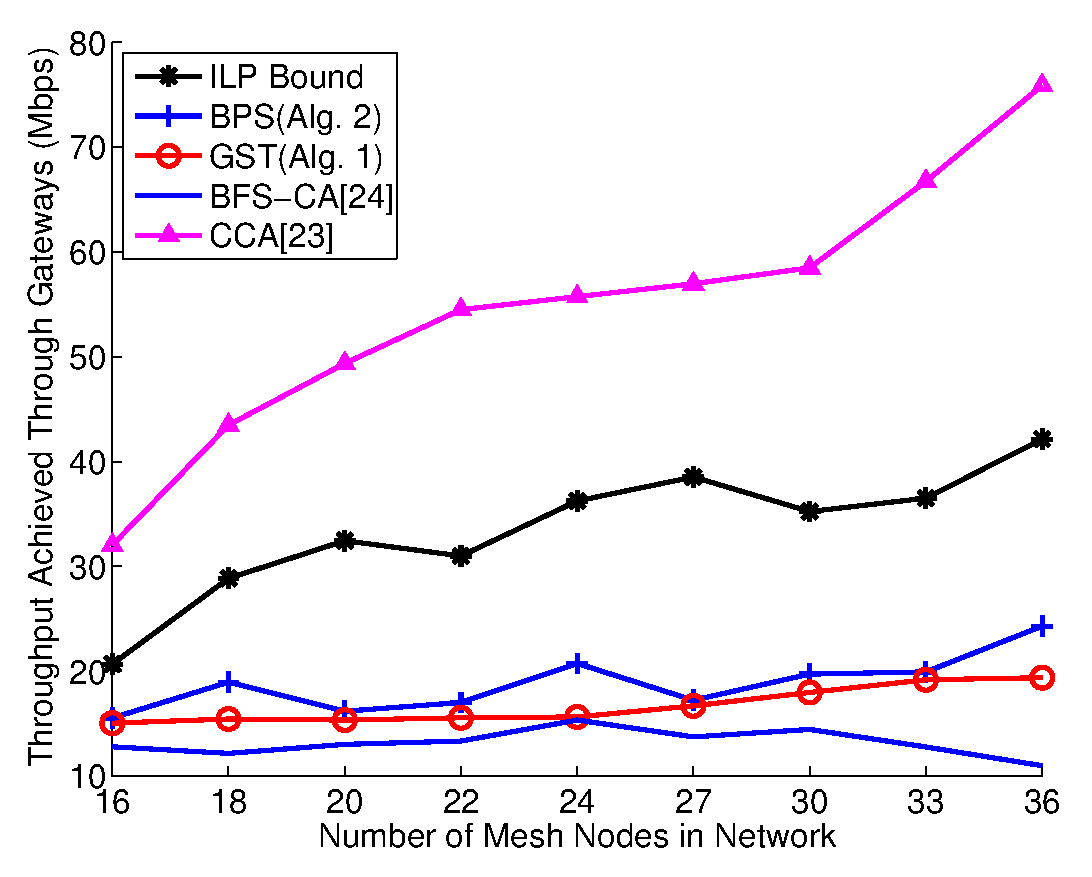
\includegraphics[width=74mm]{figures/varysize}
\vspace{-0.1in}
\caption{Max Tpt of Network Size}                                                                               
\label{fig:varysize}
%\vspace{-0.0in}
\end{figure}

\subsection{Min Conflict Weight}

~\emph{Conflict Weight} is the amount of links interfered by a single link ~\cite{JaPaPaQi03}. 









